\documentclass[a4paper,fleqn]{article}
\title{Behavior Analysis of Elderly using topic models}
\author{Kristin Rieping}
\usepackage[latin1]{inputenc} %andere lettertype
\usepackage{amsmath} %math symbols
\usepackage{amsfonts} %andere font maar wel math symbols
\usepackage{amssymb} % nog meer symbolen
\usepackage{graphicx} %plaatjes toevoegen
\usepackage{fullpage} %minder witte rand
\usepackage{cite} %voor het citeren
\usepackage{caption}
\usepackage{subcaption}

\begin{document}
\maketitle
\pagebreak
\tableofcontents
\pagebreak

\begin{abstract}
In this thesis two novel variations of the Latent Dirichlet Allocation (LDA) model are presented. The models give the opportunity to detect patterns in multi-dimensional data in an unsupervised manner. LDA-Gaussian is a combination of a Gaussian Mixture Model and a LDA model. Here the multinomial distribution of the topics, that is normally used in the LDA model, is replaced by a set of Gaussian Distributions. In this way similar looking sensor data is automatically grouped together and captured in the same topic.
LDA-Poisson, the second variation of the model, takes a set of Poisson Distribution for the topic descriptions. This distribution makes it possible to handle discrete multi-dimensional data. The parameters of both models are determined with an EM-algorithm.
Both models are applied to real sensor data, which is gathered in the homes of elderly people. It is shown that meaningful topics can be found and that a semantic description of these topics can be given.


% The goal of this algorithm is to find topics that describe the data in a way, so that it is easily interpretable and usable for different kinds of machine learning techniques that can predict different behaviors.
\end{abstract}


%----------------------------------INTRODUCTION--------------------------------------------
\section{Introduction}
% START bekijken 
The life expectancy of people is assumed to rise continuously \cite{4864}. So the percentage of elderly also increases. This means that
The world population increases unceasingly and besides the percentage of elderly also increases. The manpower to take care of elderly is diminishing. So it becomes more and more important to give elderly the opportunity to live on their own and be more independent of health care. It might be important to monitor elderly in their homes in order to give an alarm if an accident happens or to detect physical and mental declines.

Systems should detect accidents or monitor people over a longer time period, so that changes in the behavior can be found, that may 
People like to live on their own \cite{Cavallo:1315167}.
% ENDE bekijken

% START algemene omschrijving van monitoring elderly
New techniques give the possibility to monitor elderly from the distance or even automatically. These systems give the possible to detect accidents, if a person 

Some of these techniques use cameras that are placed in the homes of elderly. But these methods are privacy-sensitive and often not adopted by the elderly. Less intrusive methods use simple sensors like motion sensors or pressure mats that are placed in the homes of people.

Other methods use motion sensors that are placed at different locations in the homes of elderly. %find some example
Reading and interpreting this sensor data is often difficult and that is why often activity recognition is done to make the data more readable. But different approaches show that this is also a though challenge.
With many Machine Learning techniques it is also often the case that a lot of annotated data is required.  But the task of labeling a data set is time consuming and can also influence the output of the data while doing so. That is why unsupervised techniques are preferable. Apart from activity recognition we deal with the problem of the representation of the data. From simple motion sensors we receive binary, time sequential data, that is gained over some period of time in the homes of elderly. There are a lot of sensors placed in the houses, which leads to high-dimensional data, that is hard to interpret for classifying algorithms as well as for humans. Finding a correct representation is a challenge.\\
% ENDE algmene omschrijving

% START wat doe ik in deze thesis
In this thesis we develop an unsupervised algorithm that detects patterns in the data automatically.
In a first step, which is inspired by~\cite{farrahi2008daily}, real live data is used to build a topic model. In a second step a genetic algorithm is used to find the best representation of the data according to the likelihood that is gained from the topic models found in the first step. 
 A topic model in combination with a genetic algorithm might lead to a representation of the data that gives the opportunity to interpret the data more easily and also finds behavior patterns in the data automatically. This furthermore makes it possible to detect deviations in the behavior over a longer period of time. The data that we use is received in the same way as described in ~\cite{van2010activity}, except that our data is not annotated.\\
% ENDE thesis omschrijving

% START topic omschrijvingen
Topic models are usually used in the field of document classification. The idea is that every document might belong to a couple of different topics and a topic can be described with a distribution over words. A newly seen document can than be assigned to some topics according to the words that occur in the document. The document is than described with a distribution of topics. The topics of a model can be found in an unsupervised manner.
We use this idea to find topics in the given sensor data. So that a day in a persons life can be described with a distribution over topics. And a topic will be described with a distribution over observations. An example of a topic might be 'going to the toilet' or a more global example is 'getting up early'.\\
%%%%%%%%%%%%%%
%Hier nog even kijken
Our data differs from the data that is normally used for this kind of models in some way. For text classification the 'bag-of-words' model is often used, where a distribution of the frequency of words is built. This model is not so easily applicable to the given sensor data, because of the multidimensional and the continuous description of the data. A Text document usually does or does not contain a word of a given dictionary. Therefore our data needs to be discretized in some way.\\
%%%%%%%%%%%%
In a first approach we first simply count the amount of times that a sensor is triggered in a certain window of time. This still produces a broad variety of observations and that is why we cluster the observations with k-means, so that we are able to use the topic model 'Latent Dirichlet Allocation' described in~\cite{blei2003latent}, on our data.\\
In a second approach we develop a topic model based on LDA that models the clusters in the model itself with a Gaussian distribution in every dimension of the observation. In this way the topic model is able to handle high dimensional data. The model parameters are found with an EM-procedure, which uses the likelihood of the model to converge to the optimal model parameters.\\
\\
In the second part of the thesis we use a genetic algorithm to find the best representation of the data.
Earlier we described the part of discretization the data in some way. Choosing the correct length of a time-interval, in which the sensor activities are counted, might be hard. There are also plenty of other variables to choose, that lead to a different representation of the data. For example we can choose to group all sensors together that are in the same room of the house. But we cannot be sure that this leads to a better representation of the data. Further there are different kind of sensors placed in the houses and we might want to distinguish between these sensors, so that a different weight is given while counting an activity. For example an activity at a door sensor might give more information of a persons behavior then a motion sensor, which is triggered more often also by small, not that important movements. It might also a good idea to look at the transition of the observations, so given an observation, what are the observations before and after this one.\\
So the representation of the data depends from a lot of different variables. This variables are optimized with a genetic algorithm. The log-likelihood, from the previously derived topic models, is used as the fitness function of the genetic algorithm.\\

% START outline verslag
In the next chapter of this thesis we give an overview of related approaches. In section \ref{sec:DataDesc} we describe the data that we use in more detail. This is followed by section \ref{sec:TopicModels} which describes the two different ways of the usage of Topic Models with our data. In section \ref{sec:features} we describe the different ways of feature representation of our data. The section \ref{sec:Experiments} we describe the different experiments that we performed. In section \ref{sec:Disc} we discuss our outcomes and finalize the report with the Conclusion in section \ref{sec:Conc}.
% ENDE outline verslag



%  Instead of a bag-of-word model that describes our data, every observation is model with a Gaussian Distribution in every dimension.
% 
% 
% In a second step a genetic algorithm is used to find the best feature representation of the data. The data is discretized in times-slices and divided into different fields. The likelihood of the EM-algorithm of the topic model is used as a fitness function. In this way the best representation of the data can be found.\\ 
% Ik weet nog niet hoe ik dat precies doe, dus maar nog niet meer omschrijven.
% Together this two steps might give a good indication how this kind of data can be efficiently used with other machine learning techniques.
% This data also might give valuable information to health proffesionals. The topics described in the first step might give a good indication of the health of the elderly.
% 
% It might be possible to predict the health of a person and give additinal health care if needed.
\pagebreak


%----------------------------------------------------------RELATED WORK-----------------------------------------------------------------

\section{Related Work}
% The story line:

%%%% Monitoring the health of elderly people is done in different ways. Different type of sensors and different types of models are used to see if the people are still healthy (What does monitoring the health of elderly people include?): Give example on very global monitoring (misschien dat dit ook meer referenties zijn die in de intro terecht horen, maar je kunt ze ook vaker noemen)

%%%% A lot of systems focus on activity recognition, because the activities that people still can do give an indication how fit people are. Supervised method are often used: Describe methods that use supervised methods for activity recognition

%[(later opnoemen, omdat dit niet over oude mensen gaat maar meer in het algemeen activity recognition)Wilson \& Atkinson(STAR)]

%%%% Also semi-supervised methods are used:

%%%% The task of annotation can influence the behavior of the people that are monitored and so they not might give good data. The topic model LDA find in an unsupervised way pattern in the data. The topics can be compared to activities that needs to be founded. LDA is used on different type of data and is also applied in different kind of ways. Ga van algemeen activity recognition in huizen over na activity recognition van sensor data.
%[(gaat niet om oudere maar om activity recognition)Castanedo, they also give a nice overview how LDA is used in different kind of fields especially for activity modelling]



Monitoring the health of elderly can be done in many different ways. There exist many various approaches. Systems are developed and also implemented in houses of people to monitor mental and physical health. In \cite{Tamura1998573} a system is described that is installed at peoples home. This system focuses on solitary elderly people. They use a variety of sensors and the system can give a detailed information of the health condition of the inhabitants. Sensors where added in bathtub, toilet and bed. These devices where specially build for the experiments which makes this approach quite expensive.\\
% In \cite{Nagai2010204} a system is describes that uses cameras in the homes of people to monitor their health condition. If an emergency occurs staff can handle appropriate. Also family members have access to the video streams and can report accidents.
In \cite{Kwon20125774} more simple sensors are used to monitor the health of solitary living people. Different sensors in the houses are tracking the health condition and the system is able to automatically contact emergency services or give the signal to send a caretaker at the home. A combination of static and wearable sensors is used, some of these sensor record automatically and other needs be triggered by the inhabitant.\\
Systems that monitor the health of people need to be not intrusive, which means that the choice of sensors becomes important. People to not want to feel watched all the time, which makes the use of camera or microphones (\cite{Nagai2010204}, \cite{Wu_2003_4676}) mostly not eligible.
It is also desirable that sensors are low in cost. Another thing that is desirable is that the system collects data automatically. Inhabitants do not want to need to interact with the system constantly and the system should not affect their daily living. To meet these conditions several researchers focus on the task of activity recognition with simple sensors.\\

To make the recognition of abnormalities on short or long term behavior monitoring possible, most system rely on activity recognition. In \cite{Hong2009236} a system to recognize activities is introduced that is bases on ontolgies. Simple binary sensors, like movement sensors, contact switches and pressure mats, are used. Activities are described with ontolgies that are build from the sensor data.
In \cite{Tapia04activityrecognition} contact switches that also generate binary data are used. A naive Baysian Network is trained with using annotated data, that is received from the inhabitants of two different houses.


All the work that is described above about activity recognition uses a supervised manner to detect activities in the data. Annotating the data has some disadvantages as it is pointed out in the work of Chikhaoui et al. \cite{journals/percom/ChikhaouiWP12}. They use the topic model LDA in combination with sequential pattern mining. These sequential patterns build the words, that are needed as input for the LDA model. The found topics are comparable to the activities of previous approaches of activity recognition.
Topic models give a great opportunity to find activities in an unsupervised way.


Activity recognition is mostly done supervised, as it is done in the previous works. A topic model, often used for document classifaction, is an unsupervised model that gives the oportunity to find topics. These topics are comparable to activities. \cite{journals/percom/ChikhaouiWP12} presents a model that uses LDA to find  


A way to do activity recognition in an unsupervised way, like it is done in this work, is the use of topic models. 





Activity recognition plays a big part in health monitoring. in ... this is done with cameras. Less intrusive sensors are used in the work of ...

Different type of sensors and different types of models are used to find behavior patterns in data


Topic models give a good oportunity to find patterns in the data in an unsupervised way. Topics are found and can be related to 


%------------------------------------------------------------OLD----------------------------------------------------
% In this section an overview of related work is given. The focus is put on work that uses a similar approach but also work that uses similar data.\\
% \\
% In the work of Casale \cite{Casale:2009} continuous data is modeled with the topic model LDA. They have sensor data available gathered from wearable sensors. The words for the topic models are generated through clustering the data beforehand. Two different cluster methods are used, K-means and mean-shift. They show that applying topic models to sensor data is possible.\\
% \\
% Castanedo et al \cite{EXSY:EXSY12033} apply a LDA model to learn behavior patterns of sensor data that is gained in an office environment. They apply the Bag-of-word model to the data. A lot of data is available.\\
% \\
% Similar data and model is used in the work of \cite{journals/percom/ChikhaouiWP12}. They have data that is gained of sensors in a home environment. The data contains a brought variety of sensors, that are placed at different locations and objects. They also use the LDA model and compare it to other models as Hidden Markov Models and Conditional Random Fields. The available data is annotated which makes it possible to evaluate the topic model and compare it to other models.\\
% \\
% In the work of \cite{Huynh:2008:DAP:1409635.1409638} also wearable sensors are used to create the data. The LDA model with a Bag-of-words approach is applied and compared with the annotation of the data. It is checked if the topics that are found start end stop at the same time that an activity is annotated.\\
% \\
% Tapia et al. \cite{Tapia04activityrecognition} uses similar data. A Baysian Network is applied to the annotated data.
 



\pagebreak


%--------------------------------DATADESCRIPTION--------------------------------------------
\section{Data Description}
\label{sec:DataDesc}
In this section we describe in what kind of houses the data is gathered and what kind of persons live there. We describe the sensors that are used and give an impression of the data that is received from these sensors.
\subsection{Homes and persons}
In the homes of five different people sensors are installed. The floor-plan of these homes is for all residents the same and is shown in figure \ref{fig:floorplan}. There might be small differences of the locations of the sensors due to the personal arrangements of peoples stuff.
The persons that live in the homes are people that need healthcare on a regular basis, they are further able to live on their own. The amount of data collected differs for the different houses, but there is at least 63 days of data available for every house.

\begin{figure}[h]
\centering
 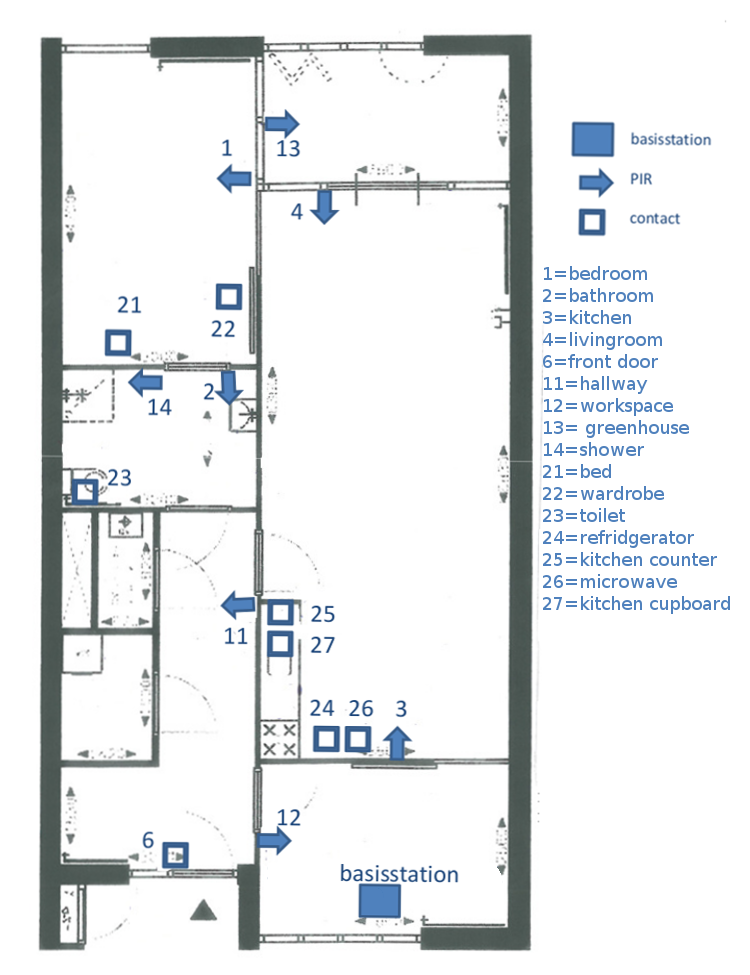
\includegraphics[width=0.7\textwidth]{Pictures/floorplan.png}
 \caption{Floorplan of the houses with sensor descriptions}
 \label{fig:floorplan}
\end{figure}


\subsection{Sensors}
There are different types of sensors installed in the homes. The contact switches are mostly installed at doors and cupboards. They get the value 'one' if a door is opened and the value 'zero' if the door is closed again.
The motion-sensor (PIR) are placed at different places in the homes, mostly against the walls. They have a range of 5 meters. If a motion occurs in the region the sensor sends an impulse value, which means that the value becomes 'one' and immediately 'zero' again . After that the sensor is set to mute for about 3 minutes, which means that in this time there is no motion captured. In this way constantly firing of the sensor will be avoided. Every activity of the sensors is send to the basis-station 3 times, so that the chance is reduced that the data is not received. The sensor system is active 24 hours. However failure can occur due to network problems, sensor failing or other unexpected problems.

\subsection{Received Data}
In figure \ref{fig:PlaineSensorData} the data stream of two different hours of one day is shown. The data belongs to one person. Several sensors that are located in the same room are manually grouped together in a field. The fields are $\{$'kitchen', 'living room', 'bathroom', 'bedroom', 'hallway'$\}$. They are marked in the figure with different colors.

\begin{figure}[h!]
  \centering
  \begin{subfigure}[b]{0.45\textwidth}
    \centering
    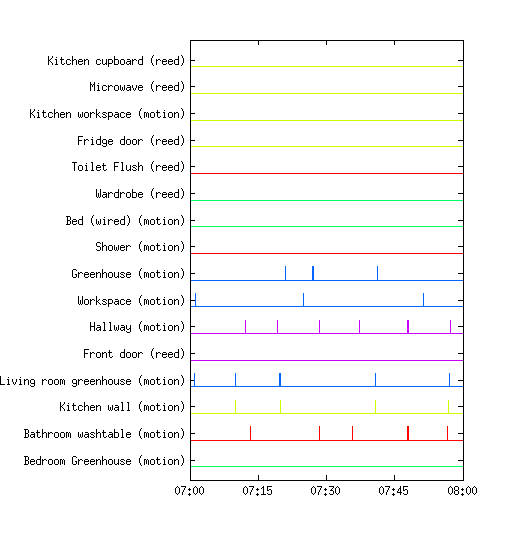
\includegraphics[width=\textwidth]{Pictures/SensorsMorningHN3Day34.png}
  \end{subfigure}
  ~
  \begin{subfigure}[b]{0.45\textwidth}
    \centering
    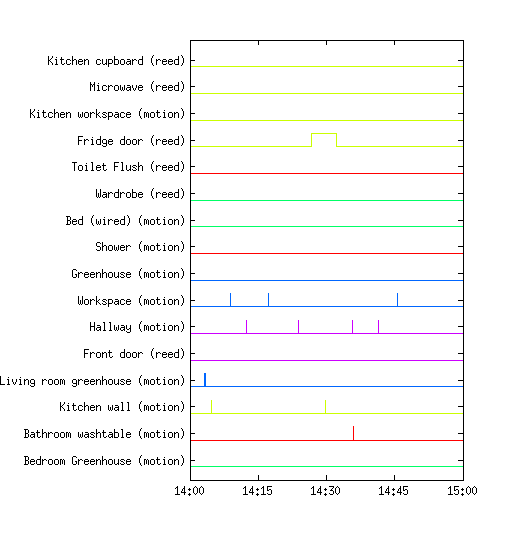
\includegraphics[width=\textwidth]{Pictures/SensorsNoonHN3Day34.png}
  \end{subfigure}
  \caption{Sensor Data for two different hours at a day of one person. The fields `kitchen`,'living room','bathroom','bedroom','hallway' are marked with the colors 'yellow','blue','red','green','purple' respectively.}
  \label{fig:PlaineSensorData}
\end{figure}

In the figure you can see the different type of data that is generated by the different sensor types. The fridge sensor is a reed sensor which has the value '1' for a longer period of time, when the door is opened for a while. The motion sensors on the other hand only give a impulse value as mentioned before. You can also see that some sensors are not triggered at all in the given time intervals.


\pagebreak

%--------------------------------------FEATURES----------------------------------------------
\section{Features}
\label{sec:features}
% WHAT DO WE HAVE?
The data that is received from the sensors generates a continuous data stream for every sensor. A good feature representation of the data is required so that the LDA model can be applied.
First the data is divided into five fields and all the sensors in one field are grouped together. In this way the data to is reduced to five dimension. The continuous data stream cannot be used as input for the LDA model. That is why the data is divided into time-slices of length $l$. If for example the length of the time-slices is $l=30$ min., the number of time-slices on one day is $n=48$.
A day starts and ends at 3 a.m. in the morning. In this way the chance to cut between activities is reduced. It still can occur that a person goes to bed late or that he needs to visit the toilet. For now this fact is left out in the part of modeling.\\
\\
In every time-slice of a field we look at the amount of times that a sensor in this field is activated and count this activities. So we do not look at the length of time that a sensor stays in the active state, but only how often it changes into the active state. So given five fields every observation $o_n$ has five dimension with integer values.
We do not take the length of the sensor activity into account because this sometimes can lead to unrealistic high values. These values can occur if someone leaves a door open of a cupboard for example. Then the observations contains a high value but does not contain a lot of information about the behavior. In figure \ref{fig:FeatEx} we give an example how the data is translated into a vector representation for one time-slice.%Give an example.

\begin{figure}[h]
\centering
\begin{minipage}{0.55\linewidth}
\centering
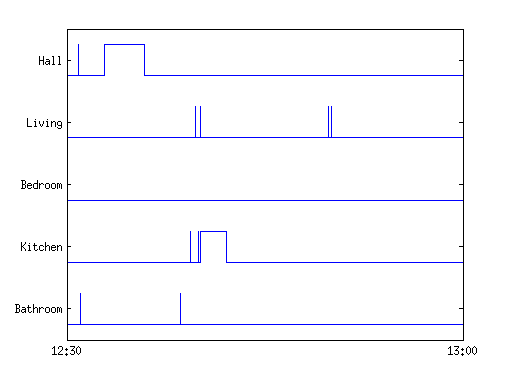
\includegraphics[width=\textwidth]{Pictures/FeatExample.png}
\label{fig:FeatEx}
\end{minipage}
\begin{minipage}{0.35\linewidth}
\centering
\begin{equation*}
 \begin{bmatrix} 
 o_{Hall}\\
 o_{Living}\\
 o_{Bedroom}\\
 o_{Kitchen}\\
 o_{Bathroom}
 \end{bmatrix}
 =
  \begin{bmatrix} 
 2\\
 4\\
 0\\
 3\\
 2
 \end{bmatrix}
\end{equation*}
\end{minipage}
\caption{Vector representation of the data. The data of the sensors is shown in the left image. It is translated in the vector shown on the right-hand side.}
\end{figure}

An additional dimension for the time is used. There are two different ways how the time dimension is added to the observations. The fine-grain representation adds the number of the time-slice in which an observations is captured, at the end of the observation vector. In the coarse-grain representation the 24 hours of a day are divided into the five time intervals $\{ 3am - 8am, 8am - 1pm, 1pm - 18pm, 18pm - 23pm, 23pm - 3am  \}$. So the observation of figure \ref{fig:FeatEx} will become $o_n=\{2,4,0,3,2,2\}$ in the coarse-grain representation. The observation falls into the second time interval. In the fine-grain representation the observation will be $o_n=\{2,4,0,3,2,20\}$ if the total number of time-slices on a day is $n=48$.\\

The given feature representation, with the two variation of the time dimensions, are used in the following chapters. But there are plenty more ways to describe the data so that it can be used in the LDA model. For example the size of the time-slices can be changed. This leads to a higher resolution and may give more detailed information of the behavior.
Another way to get a different feature representation is to combine sequential time-slices as it is described in the work of Farrahi et al. \cite{farrahi2008daily}. So for a given time-slice add the observation values of the previous and the subsequent time-slice. This will lead to a 15 dimensional observation plus one dimension for the time value. In this way the transitions are taken more into account, which might contain valuable information over the behavior.\\
We also might want to combine different sizes of time-slices into one observations, so that the global and detailed view is combined.\\
The different kind of sensor are also maybe important. The reed sensor, which is mostly installed at doors might contain more important information than the motion sensor. The motion sensor is also triggered by small movements, whereelse if a door is opened from a cupboard you can assume that an important action has taken place, as for example the person is grabbing a plate to prepare a meal. So it might be an idea to give a higher weight to sensor activities of reed sensors in house.\\
It is obvious that the feature space can be made nearly infinity big and it is quite a challenge to find the best feature representation. The likelihood that is gained from the EM-algorithms might be a good indication for a good feature representation.

% % Wat hoort hier in te staan???
% - data wordt ingedeeld in fields, deze is afhankelijk van de locatie van de sensor
% - alle observaties in een field worden samen bekeken
% - een dag wordt ingedeeld in timeslices
% - the amount of timeslices is variable
% - we count the amount of 1's in one timeslice of a field
% - there are a lot more different ways to use the data
% - we can combine different timeslices, so maybe the best topics are found if their are different timeslice widths are combined.
% - another way to combine the timeslices is to look at the previous and the subsequent timeslice and combine the three observations of this timeslices into one big observation. In this way the transitions are captured well.
% - We also may want to look at the way the different sensors in the homes are handled. A reed sensor might be much more important than a motion sensor. The reed sensor is mostly connected to doors and opening the fridge might be of more information than if a person only moves in the living room, this might be only be caused by someone who shifted a little bit on the couch. 
% 



% In a first approach we discretize the data into time-slices of half an hour. In each time-slice we count the amount of sensor activations in all the fields. We differentiate between two different kind of sensors. For the reed sensors, which are installed at doors and the toilet flush, we count every change of sensor value. So open and close a door is both count as an activity.\\
% %How is the toilet sensor been seen? 0 and 1?
% The motion sensor can sens a new motion every minute. But in between the sensor will still have the same value, which is 1. That is why we count for every minute the sensor has the value 1 a new activity. So if the sensor has the value 1 for three minutes, we count three activities for the particular sensor.\\
% The amount of activities captured at every sensor is add together for every field. So every time-slice can be represented as a vector $w_n$ of length five, for every field a value $v_i>=0 \in \mathbb{N}$. We add an additional dimension to the vector to capture the the time in which the observation is taken. The values lay between 1 and 48, for every time-slice a value. This is necessary to model the time dependency from the data, which is not automatically captured in the topic model that we are going to use. We say that a day starts at 3 a.m. so that we reduce the chance to cut between activities. It still can occur that a person goes to bed late or that he needs to visit the toilet, but we will ignore this fact for now.
% 

\pagebreak

%-----------------------------------TOPICMODEL----------------------------------------------
\section{Topic Models}
\label{sec:TopicModels}
In the introduction of this section we describe the general idea of topic models followed by a section that describes how this kind of models can be used on the sensor data that we have. After that we introduce the extension of the LDA model which combines the clustering and topic estimation in one algorithm. And after that LDA-Poisson model is described.

\subsection{Introduction to Topic Models}
Topic models are often used in the field of document classification. Given a set of documents (corpus) it is assumed that every document belongs to one or more topic(s). So for example a news article may belong for some percentage, let us say 30 \%,  to the topic 'Economy' and for 70 \%  to the topic 'Politics'. Another document of the same Corpus may belong to the topic 'Economy' with 50 \%, 'Politics' with 30 \% and 'Global Warming' with 20 \%. There might be a lot of different topics and the topics can have different level of details. 
\\
The topics are defined by several words that can occur in the documents. The topic 'Economy' may be defined by the list of words \{'trade', 'industry','GDP'\}. Other topics have different lists of words that describe them. The list might be longer or shorter and the words in the list will depend on the corpus that is used to generate the topics. It might also be the case that one word belongs to multiple topics. Eventually we can find the topic distribution of a document according to the words that are included in this document.\\
In the topic model 'Latent Dirichlet Allocation' (LDA) it is assumed that a Corpus can be made out of a generative process. The parameters that generate the corpus are than used to describe the model of the corpus. The generative process which builds a corpus is as follows:
\\
For every document that is generated in the Corpus
\begin{enumerate}
 \item Choose the amount of words in the document from $N~Possoin(\xi)$.
 \item Choose a topic distribution $\theta \sim Dir(\alpha)$ for the document.
 \item For each of the N words $w_n$:
 
 \begin{enumerate}
  \item Choose a topic $z_n \sim Multinomial(\theta)$.
  \item Choose a set of words $w_n$ from the set of all words $V$ from $p(o_n |z_n;\beta)$, a multinomial probability conditioned on the topic $z_n$. Where $\beta$ is the distribution over words given a topic.
 \end{enumerate}

\end{enumerate}

The model is also shown in figure~\ref{fig:modelBasic}. The parameters $\alpha$ and $\beta$ define a corpus.

\begin{figure}[h!]
\centering
\def\svgwidth{400pt}
\input{Pictures/ModelBasic.pdf_tex}
\caption{Graphical representation of the LDA model}
\label{fig:modelBasic}
\end{figure}

To determine the model parameters an EM-algorithm can be used. How this algorithm can be applied is extensively described in~\cite{blei2003latent}. \\
In the next section we describe how this model can be used with the sensor data, that is gained in the different houses.


\subsection{Topic models with Sensor Data}

In order to employ the topic model with the sensor data we first introduce the different levels of description given our data and relate them to the terms of document classification.
\begin{itemize}
 \item \textbf{Dataset/Corpus}: One dataset $C$ describes the sensor data that is gained in the home of a single person. So for every person there is a separate dataset. This set of data can be compared with a Corpus in document classification.
 \item \textbf{Day/Document}: Every Dataset is divided in days. A day can be compared with one document in a Corpus.
 \item \textbf{Observations/Words}: Finally every day is build of a set of observations. The amount and dimension of the observations depend on the representation of the features, which is described later in chapter \ref{sec:features}. Observations can be roughly compared with words in document classification.
\end{itemize}

There are some differences between the data that is used for topic detection in documents and our sensor data.\\
The main difference is that words that look similar to each other, like "illusion" and "allusion", may belong to a totally different topic in the document classification. But in our case, two observation that are similar to each other, are more likely to refer to the same topic. So for example if the topic "preparing food" has the observation using fridge 3 times in it, an observation of using fridge 4 times may also refer to the same topic. That is why we cannot directly compare the words in a text document with the observations used in the sensor data.\\
Another difference is that in the topic model, LDA, it is assumed that the order of the words, in that they appear in the text, does not matter. In our case the time when an observation is made is of big influence. We can overcome this problem by adding time as an additional dimension to our observations.
\\

If the Bag-of-Words model will be applied to the data, a dictionary of all unique observations must be made. All this observations then will can be seen as a different dimension which are independent of each other. In figure~\ref{fig:FSBOW} it is shown how the BOW is used!!!!!!!!!. Observations that are assigned to the same topic do not need to lie close to each other in the feature space and the correct topics might not be found with LDA. This approach needs a lot of data to find meaningful results. The size of the 'dictionary' varies depending on the feature representation. 

\begin{figure}[h!]
\centering
\begin{subfigure}[b]{0.3\linewidth}
\centering
\def\svgwidth{140pt}
\input{Pictures/BOW.pdf_tex}
\caption{The Bag-of-words model with topic assignment.}
\label{fig:FSBOW}
\end{subfigure}
~
\begin{subfigure}[b]{0.3\linewidth}
\centering
\def\svgwidth{140pt}
\input{Pictures/kMeans.pdf_tex}
\caption{Feature space with k-means and topic assignment.}
\label{fig:FSk-means}
\end{subfigure}
~
\begin{subfigure}[b]{0.3\textwidth}
\centering
\def\svgwidth{140pt}
\input{Pictures/GMM.pdf_tex}
\caption{Gaussian Mixture Model with LDA}
\label{fig:GMM+LDA}
\end{subfigure}
\caption{The two different topics are marked with red and blue.}
\end{figure}

To make sure that similar observations will be grouped together and will appear in the same topic, we can apply the k-means algorithm to find clusters in the data. The centroids of the clusters then function as 'words' and can be used in the same way as text data. So if we apply LDA to the clustered data some clusters may fall into the same topic. This is shown in figure ~\ref{fig:FSk-means}.\\
The outcome of the LDA model does strongly depend on the outcome of the apriori used cluster algorithm. The clusters that are found with k-means are maybe not a good representation of the data. All clusters may have the same amount of influence on the LDA model, which might not be the correct way to describe the data. The Gaussian Mixture model might give a better description of the clusters. Combining the part of clustering directly into the topic model will avoid the apriori clustering and the clusters are then formed due to the topics, which will give a better globalization of the data. In figure \ref{fig:GMM+LDA} we show how the combination of the part of clustering into the Topic Model might improve the Gaussian Mixture Model.\\
According to the feature representation, which in our case is a discrete derivation of the sensor data, a Poison distribution might be a good choice to model the topic distributions. The Poisson distribution can be used instead of the Gaussian distribution.



% 
% Let us say we have a two dimensional feature space. For example we only have two sensors in our data, than every dimension will refer to one of the sensors. A representation of this model is shown in figure bla (a). A cross marks an observation and is seen as a new 'word' in the bag-of-word method. We can use this data with the LDA model. The problem only with this approach is that similar observations are not group together and it might be possible that a similar observations are not grouped together in the same topic when we apply the LDA model.

% 
% 
% If we cluster the observations on forehand with a the k-means algorithm we can reduce the size of the dictionary (which contains all unique observations) and use again the LDA method to find the topics. The problem here is that there is a hard separation line between the clusters as is shown in figure bla (b).
% 
% So we invented a third method which is a kind of gaussian mixture model included into the LDA topic model. So instead of cluster the model with priors from the data itself we relate the priors directly to the topis and combing the part of clustering and the deriving the topics in one algorithm. In this way clusters are grouped together directly if they belong to the same topic, as is shown in figure bla (c).
% 
% 
% 

% 
% 
% In the next two sections we describe the two different ways how we use the topic models with our data. First we describe the combination of k-means clustering and the basic LDA model as it is described in [Blei]. And after that we describe our new approach that combines the clustering and topic modelling in one algorithm. In this algorithm we step away from the bag-of-words model representation of the data.
%  Nog toevoegen dat we twee manieren gaan gebruiken(LDAbasic and LDAext)
% %%TOT HIER!
% 
% 

%   \subsubsection{K-means}
%  In the previous section we addressed the problem of a wide variance of observations. With a bag-of-words model, as it is used in the LDA approach, similar looking words/observations are not likely to be put in the same topic. All observations, that are not exactly the same, are independent from each other and may not lead to the same topic. Because of the low amount of training data it is not very likely that the same observation will be seen often enough to learn topics from the data properly.
% That is why we need to reduce the amount of unique observations and group similar observations together. In terms of document classification, we could say that we need to reduce the size of the dictionary.


% In a first-approach we use k-means clustering to reduce the size of the dictionary, which is the set of all observations that can be found in the data.
% We do not use the time dimension for the clustering part, because this would compromise our data so that clusters are not detected properly. We use the euclidean distance to determine the best mean.
% 
% maybe preprocess the data with coarse grain time dimension
% 
% size of the dictionary
% is it the case that with a lot of data simialar looking words will be put in the same topic? Or will it just be a different topic?
% 
% 
% 
% In our data the size of the dictionary, which contains all unique observations in the whole corpus is relative large with respect to the size of the data that we have. There are a lot of different observations that are similar to each other, but differ only in one value of the 6 dimensions. So for example the observation $o_1=\{1 ,2 ,5 ,3,14\}$ is similar to the observation $o_2=\{2 ,2 ,5 ,3,14\}$. The only difference of sensor activities is in the first field. In the LDA model these two observations/words will be seen as two different dimensions and the similarities are not captured. In fact a lot of words will only be seen once in the whole corpus and finding good parameters is not possible.
%  So we need to find a way to capture similar observations to build a proper topic model. A simple way is to cluster all observations together and then use the EM-algorithm to estimate the parameters of the  LDA model.
%  For the clustering part we used the k-means algorithm. We reduced the size of the dictionary to 20. After that we use the EM-algorithm as described above.
%  In the clustering we leave out the time dimension because this is fucking up the clusters
 
%   \subsubsection{Latent Dirichlet Allocation with clustered Data}
% The generative model 'Latent Dirichlet Allocation' [Blei] is a way to describe a topic model. In this model it is assumed that a Corpus can be generated from a distribution of topics, where every topic can be represented with a distribution of words. In our case the documents are days and the words are observations $o_n$. In the previous section we described how we reduced the size of the dictionary $V$.
% The generative process that would create the data will look like this:
% 
% For every day that will be generated:
% \begin{enumerate}
%  \item Set the amount of observations in every document to size N (for every day the same amount).
%  \item Choose a topic distribution $\theta \sim Dir(\alpha)$ for the day.
%  \item For each of the N observations $o_n$:
%  
%  \begin{enumerate}
%   \item Choose a topic $z_n \sim Multinomial(\theta)$.
%   \item Choose a set of observations $o_n$ from the set of all observations $V$ from $p(o_n |z_n;\beta)$, a multinomial probability conditioned on the topic $z_n$. Where $\beta$ is the distribution over observations given a topic.
%  \end{enumerate}
% 
% \end{enumerate}
% %!!!Describe the model variables!!!!!
% 
% With the assumption that the data that we got from the sensor system has the same structure than the data created with the generative process we can find the model parameters $\alpha$ and $\beta$ for LDA with the EM-algorithme described in \cite{blei2003latent}.

\subsection{LDA-Gaussian Model}
In this section we explain how the part of clustering is combined within the LDA model itself. Instead of the k-means clusters we use a Gaussian distribution to model every dimension within the features.


\subsubsection{Motivation and Assumptions of the Model}
 
Using the cluster algorithm k-mean in advance has some disadvantages. First of all we need to choose the amount of clusters. This is not always that easy and then it is still not assured that the best clusters are found. Every cluster also has a strict separation line, which does not give any degradation if a value is far away from the mean of the cluster. There is no quality measurement of the clusters given. So every cluster is even probable to occur in the topic model, which is not always desirable.

With a Gaussian Mixture Model we might be able to distinguish between more or less important clusters. But we might want to let the topic model decide which topics have more influence and which have not, according to the data.\\
That is why we combined the clustering part and the topic estimation into one step. Instead of a multinomial distribution over all observations that occur in the 'Dictionary', we model a Gaussian distribution over every dimension of the observations. In this way similar observation can be captured in the model itself and are not generalized in one cluster beforehand.\\
The difference is that instead of a large, fixed set of unique observations (Dictionary), with a multinomial distribution, we take a Gaussian distribution over every dimension of the observations. In this way smoothing is not necessary, because unseen observations will be handled properly.
In the next sections we describe the model in more detail. We first give an overview of the generative process. Then we explain the variational inference that is necessary to make the parameter estimation possible. And finally explain the EM-algorithm that determines the parameters.

% Every topic will have its own distribution over the dimensions. A
% topic can be described as shown in figure %\ref{fig:topic}.
% In this figure an example of a topic description is shown
% \begin{figure}
%  \includegraphics[\width=\textwidth]{Pictures\topics.png}
%  \caption{An awesome topic}
%  \label{fig:topic}
% \end{figure}

  \subsubsection{Model Description}
  
  Our model assumes that every day in a dataset can be represented as random mixtures of latent topics, where every topic can be described as a distribution over observations. We assume the following generative procss for every day $m$ in the data set $C$:
\begin{enumerate}
 \item The amount of observations on a day $m$ is fixed with size $N$ (for every day the same size).
 \item A day has a distribution over the topics given with $\theta \sim Dir(\alpha)$.
 \item For each of the N observations on a day $o_n$:
 
 \begin{enumerate}
  \item Estimate the topic $z_n \sim Multinomial(\theta)$.
  \item An observation $o_n$ is gained from $p(o_n |z_n,\boldsymbol\mu,\boldsymbol\sigma)$,  which is a probability that can be drawn from a set of Gaussian distributions. This probability is conditioned on the topic $z_n$ and the Gaussian Parameters $\vec{\mu_i}$ and $\vec{\sigma_i}$ of length $d$ that belong to the estimated topic $i$.
 \end{enumerate}

\end{enumerate}
  
In this model the amount of topics $k$ is assumed to be known and fixed and with it the size of the topic variable $z$.
The probability for the observations is parametrized with two matrices $\boldsymbol\mu$ and $\boldsymbol\sigma$, both of size $D\times k$, where $D$ is the amount of dimensions in an observation and $k$ the amount of topics. They present the mean and standard deviation respectively and for every topic $i$ and every dimension $d$ there is a set of parameters, which describes a Gaussian distribution. Every value of a dimension for an observation $o_{ndi}$ can then be drawn from a Gaussian Distribution $\mathcal{N}(\mu_{di},\sigma_{di})$.
The size of the dimension $D$ is assumed to be fixed and a more extensive description of the representation of the observations is given in section \ref{sec:features}. $\alpha$ represents the Dirichlet parameter and is vector of length $k$.

In figure \ref{fig:modelExt} the graphical representation of the model is shown. It differs from the basic LDA model (figure \ref{fig:modelBasic}) in the description of the topic distribution $\beta$, which is here replaced with $\mu$ and $\sigma$.

\begin{figure}[h!]
\centering
\def\svgwidth{0.8\textwidth}
\input{Pictures/ModelExt.pdf_tex}
\caption{Graphical representation of the LDA-Gaussian model}
\label{fig:modelExt}
\end{figure}




  
Assuming that the generative process described above can describe the available data properly, we now want to find the parameters so that the model best describes our data. We want in fact maximize the probability for the dataset $C$ given the model with respect to the parameters $\alpha$, $\mu$ and $\sigma$. This probability looks like this
\begin{equation}
p(C|\alpha,\mu,\sigma) = \prod_{m=1}^M p(m|\alpha,\mu,\sigma)
\end{equation}
where $M$ is the amount of days within the dataset and the probability for a day $m$ given the three parameters, which is the marginal distribution over a day, is
\begin{equation} 
p(m|\alpha,\mu,\sigma) = \int p(\theta|\alpha)  \left( \prod_{n=1}^N \sum_{z_n} p(z_n|\theta) p(w_n|z_n, \mu,\sigma)  \right) d\theta
\end{equation}
This distribution is gained by integrating the joint distribution \ref{eq:Joint} by $\theta$.
\begin{equation} \label{eq:Joint}
 p(\theta,\textbf{z},\textbf{w}|\alpha,\mu,\sigma) = p(\theta|\alpha) \prod_{n=1}^N p(z_n|\theta) p(w_n|z_n,\mu,\sigma)
\end{equation}
In the next section we describe how we can find the optimal parameters for the model given a data set.


  
\subsubsection{Variational Inference}
 
The marginal distribution, which is given in the previous section, can be written in terms of the parameter $\alpha$, $\mu$ and $\sigma$ as
  \begin{equation}
   p(m|\alpha,\mu,\sigma) = \frac{\Gamma (\sum_i \alpha_i)}{\prod_i \Gamma(\alpha_i)} \int \left( \prod_{i=1}^k \theta_i^{\alpha_i-1} \right)
   \left( \prod_{n=1}^N \sum_{i=1}^k \prod_{d=1}^D \theta_i \mathcal{N}(o_{nd},\mu_{id},\sigma_{id} ) \right)
  \end{equation}
Due to the coupling between $\theta$ and the Gaussian parameters $\mu$ and $\sigma$ this probability is intractable to compute.	




That is why we use a convexity-based variational algorithm to approximate the log-likelihood of a given dataset. 
An approximation of the model is given with 
  \begin{equation}
   q(\theta,z|\gamma,\phi) = q(\theta|\gamma) \prod_{n=1}^N q(z_n|\phi_n).
  \end{equation}
In this model $\gamma$ represents the Dirichlet parameter and $\phi$ are the multinominal parameter which can be viewed as the probabilty $p(z_i|o_n)$ and is given as a $k \times N$-matrix for every day $m$. The graphical representation of the model is shown in figure \ref{fig:ModelApprox}.
  
 
\begin{figure}[h!]
\centering
\def\svgwidth{0.4\textwidth}
\input{Pictures/ModelApprox.pdf_tex}
\caption{Approximation of the model.}
\label{fig:ModelApprox}
\end{figure}
 
  
  
  
  Given the variational distribution for aproximate model we can estimate the lower bound of the log-likelihood with the Jensen inequality as
  \begin{equation}
   \begin{split}
    L(\gamma;\phi;\alpha;\mu;\sigma) =& E_q[\log p(\theta|\alpha)] + E_q[\log p(\textbf{z}|\theta)] + E_q[\log p(\textbf{w}|\textbf{z},\mu,\sigma)] \\
   & -E_q[\log p(\theta)] - E_q[\log q(\textbf{z})]
   \end{split}
  \end{equation}

In terms of the model parameters and the variational parameters this becomes
\begin{equation}
  \begin{split}
 L(\gamma;\phi;\alpha;\mu;\sigma) =& \log \Gamma (\sum_{j=1}^k \alpha_j) - \sum_{i=1}^k \log \Gamma(\alpha_i) + \sum_{i=1}^k (\alpha_i-1)(\Psi(\gamma_i)-\Psi(\sum_{j=1}^k \gamma_j)) \\
 & + \sum_{n=1}^N \sum_{i=1}^k \phi_{ni} (\Psi(\gamma_i)-\Psi(\sum_{j=1}^k \gamma_i)) \\
  & + \sum_{n=1}^N \sum_{i=1}^k \sum_{d=1}^D \phi_{ni} \log( \mathcal{N}(o_{nd};\mu_{id},\sigma_{id})) \\
  & - \log \Gamma (\sum_{j=1}^k \gamma_j) + \sum_{i=1}^k \log \Gamma (\gamma_i) - \sum_{i=1}^k (\gamma_i -1)(\Psi(\gamma_i)-\Psi(\sum_{j=1}^k \gamma_j)) \\
 & - \sum_{n=1}^N \sum_{i=1}^k \phi_{ni} \log \phi_{ni}
  \end{split}
  \label{eq:likeli}
\end{equation}
With an EM process we are then able to maximize this lower bound on the log-likelihood. The two steps are:
  \begin{enumerate}
   \item \textbf{E-step:} For each day $m$, optimize the variational parameters $\{ \gamma_{m}*,\phi_{m}* \}$
   \item \textbf{M-step:} Maximize the resulting lower bound on the log-likelihood with respect to the model parameters $\alpha$, $\mu$ and $\sigma$.
  \end{enumerate}
  
  We now give a more detailed description on both of these steps.
  
  \paragraph{E-step}
In the e-step of the algorithm the variational parameters $\phi$ and $\gamma$ are optimized. To get the update function for $\phi$ we get all terms of the lower bound of the loglikelihood in equation (\ref{eq:likeli}) that contains the variable $\phi$. 
Take $y_i=\sum_{d=1}^D \mathcal{N}(o_{nd};\mu_{id},\sigma_{id})$
We add the constraint $\sum_{i=1}^k \phi_{ni}=1 $ to the formula and get
\begin{equation}
 L_{[\phi_{ni}]} = \phi_{ni}(\Psi(\gamma_i)-\Psi(\sum_{j=1}^k \gamma_j)) + \phi_{ni} \log(y_i) + \lambda_n(\sum_{j=1}^k \phi_{ni} -1)
\end{equation}
From this equation we take the derivative of the formula and set it to zero. This leads to the first update function
\begin{equation}
 \phi_{ni} \propto \log(y_i) \exp(\Psi(\gamma_i) - \Psi(\sum_{j=1}^k \gamma_j))
\end{equation}
\\
For $\gamma$  we also take all terms of equation \ref{eq:likeli} that contain this variable and set the derivate to zero. This leads to the second update equation
\begin{equation}
 \gamma_i = \alpha_i + \sum_{n=1}^N \phi_{ni}
\end{equation}

  %Nu nog de algorithme geven

  \paragraph{M-Step}
  
In the m-step the parameters of the Gaussian distribution $\mu$ and $\sigma$ are estimated with the weighted arithmetic mean calculated over all observation in a dataset given the parameter $\phi$, which is gained in the previously e-step. This leads to the update formulas
\begin{equation}
 \mu_{di} = \frac{\sum_{m=1}^M \sum_{n=1}^N o_{dn} \phi_{ni} }{\sum_{m=1}^M \sum_{n=1}^N  \phi_{ni}}
\end{equation}
and
\begin{equation}
 \sigma_{di} = \sqrt{\frac{\sum_{m=1}^M \sum_{n=1}^N o_{dn}^2 \phi_{ni} }{\sum_{m=1}^M \sum_{n=1}^N  \phi_{ni}} - \mu_{di}^2}
\end{equation}
\\
To calculate the parameter $\alpha$ we again take all terms of the likelihood that contains the variable $\alpha$. The derivative in the Hessian form is
\begin{equation}
 \frac{\partial L}{\partial \alpha_i\alpha_j} =  m(i,j) M \Psi'(\alpha_i) - \Psi'(\sum_{j=1}^k \alpha_j)
\end{equation}
On this equation we can use the Newton-Rhapson method to calculate the optimal $\alpha$.

\subsection{LDA-Poisson Model}


If the features are described in a discrete way, which means that every dimension has an integer value, the Poisson distributions is a better choice to describe the data. In figure \ref{fig:LDAPoisson} the graphical representation of LDA-Poisson model is shown. 

\begin{figure}[h!]
\centering
\def\svgwidth{0.8\textwidth}
\input{Pictures/ModelPois.pdf_tex}
\caption{Graphical representation of the LDA-Poisson model.}
\label{fig:LDAPoisson}
\end{figure}

The variational Inference and the EM-procedure will be the same as described before, except for the Gaussian distribution that is exchanged with the Poisson distribution. The parameter $lambda$ which describes the Poisson distribution is calculated in the M-step with
\begin{equation}
 \lambda_{di} = \frac{\sum_{m=1}^M \sum_{n=1}^N o_{dn} \phi_{ni} }{\sum_{m=1}^M \sum_{n=1}^N  \phi_{ni}}.
\end{equation}



% For a reason 
% the reason is that lda captures priors for the days, that are given with the 
% which is still not is clear for me, we combine the clustering and determining of the topics in one algorithm.
% Preprocessing the data with k-means may not capture the topic distributions probably. The time dimension is not taken into account in the clustering part. So we want to avoid the preprocessing the data with k-means and add the the clustering part directly in the model.
% So first we describe how the model will change with respect to the LDA model descriibed above (or maybe: ... how extension of the LDA model looks like) and we also describe how the parameters are determined with the EM algorithm.
% 
% 
% So what is different? Maybe do not ask this question but just explain how the model looks like.
% 
% The main change of the model is that it is also captures similar observation in one topic.
%  So instead of describing a topic only with one discrete value in one dimension, we model every dimension in the observation with a Gaussian distribution. So every dimension given a topic needs to be defined with a mean and a standard deviation. The dimension might depend from each other
% 
% 
%   This is done in the following way:
% Instead of storing the probability for a observation given a topic, which is done in the matrix $\beta$, we assume that every dimension of the observations is normal distributed given a topic. So we store the mean and variance for every dimension given a topic in two matrices of size $d \times k$ where $d$ is the dimension of the observations and $k$ the amount of clusters. For now we assume that the dimensions of the observations are uncorrelated. The EM-algorithm is adjusted to calculate the $\beta$- matrix properly.
% 
% - The combination of the k-means clustering and the LDA model might not capture the topics correctly. The k-means clustering gives a hard boundaries on the words, which is also a drawback from the sequential combination of clustering and topic estiamtion. Therefore we want to comine these two step in one.



\pagebreak

%----------------------------------------EXPERIMENTEN-----------------------------------------
\section{Experiments}
\label{sec:Experiments}
In this section we describe experiments that are performed. In the section of the qualitative results we give some visualizations of the topics that are found with the different models. We show that the topics can be meaningful and that semantic descriptions can be given to some of the topics.
In the section of the quantitative results we compare the two developed models with each other and show the performance for different amount of topics and different amount of time-slices.

% Wat wil ik nou eigenlijk aantonen en kan ik dat ook aantonen?
% Ik wil aantonen dat het nieuwe model werkt. Ik wil aantonen dat het beter werkt dan normal LDA model. 
% Het is al door meerdere mensen aangetoond dat topic modellen wel van nut zijn om behavior patronen in sensor data te vinden.
% en we kunnen dus aantonen dat onze nieuwe methode OOK werkt, want we kunnen patterns vinden. eg: een dag in de week is de persoon in de middag weg, of 's nachts moet die persoon naar het toilet

% QUALITATIVE EXPERIMENTEN
%Ik wil aantonen dat mijn model werkt en dat je wel zinnige informatie eruit kunt halen. Je kunt een semantische omschrijving van de topics geven.
%We vergelijken de nieuwe method met de BOW/k-means methode we kunnen hier ook aangeven wat de verhoudingen zijn van worden in de data en unique worden die zijn gevonden. Dit geeft ook al aan dat BOW waarschijnlijk niet werkt


%Met de gegeven data en de gekozen feature representation zijn we niet in staat om zinnige informatie uit de BOW model te halen.

% QUANTITATIVE EXPERIMENTEN


% In this section we first give some qualitative results, where the topic distribution on some days are shown. 
% Then we do something else
% Then we compare the BIC's?
% And after that we make a small test according to the feature representation.


%To test the performance of the topic models we set the variables of the features to fixed values.  In the basic LDA model we use a coarse grain value for the time. This means that the sixth dimension can have 5 different values, where the time intervals are $\{ 3am - 8am, 8am - 1pm, 1pm - 18pm, 18pm - 23pm, 23pm - 3am  \}$.
\subsection{Qualitative Results}
To visualize the topics we give an impression about how the topics are distributed over the day. For the data of one house we show the topic distribution for 10 different days and compare the results for the four different models. The models are the LDA with 

of one house and mark every time-slice with a color that represents the assigned topic to that time-slice. To find the topic distribution we run the LDA algorithm on the whole data set which leads to the model parameters. With these parameters we then run the E-step again on the data set of the 10 days that are visualized. In this way we find the topic distribution on every time-slice.\\
In the following figures we used $N=96$ time-slices for a day. Every observation that is used has 6 dimension. The first five dimensions are the sensor information of the fields $\{$'kitchen', 'living room', 'bathroom', 'bedroom', 'hallway'$\}$. The sixth dimension belongs to the time, where we divided a day into the five time intervals $\{ 3am - 8am, 8am - 1pm, 1pm - 18pm, 18pm - 23pm, 23pm - 3am  \}$.

\paragraph{BOW model with and without pre-clustering}
We visualize the topic distribution on the first 10 days and initialize the LDA model with $k=5$ topics. In figure \ref{fig:bow/kMeans} we show the outcome of the LDA model with data in the form of the Bag-of-Word model and the pre-clustered data with k-means algorithm. Both algorithms are not able to find 5 distinctive topics in the 10 days.\\

\begin{figure}[h!]
 \centering
 \begin{subfigure}[b]{0.45\linewidth}
  \centering
  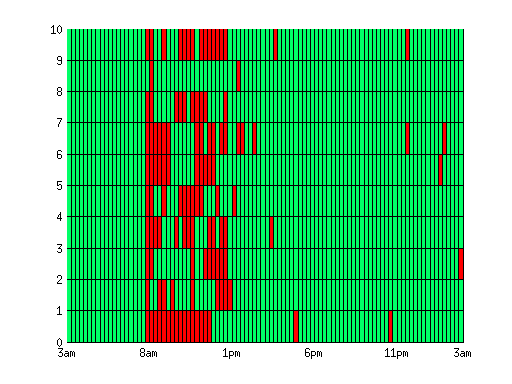
\includegraphics[width=\textwidth]{Pictures/DayTopicsTs96k5bow.png}
  \caption{Topic distribution for 10 days for the Bag-of-Words model}
 \end{subfigure}
 \begin{subfigure}[b]{0.45\linewidth}
  \centering
  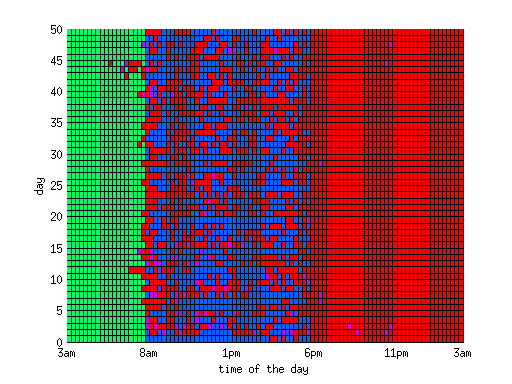
\includegraphics[width=\textwidth]{Pictures/DayTopicsTs96k5Clus.png}
  \caption{Topic distribution for 10 days for the k-means model}
 \end{subfigure}
 \caption{}
 \label{fig:bow/kMeans}
\end{figure}

\paragraph{LDA-Poisson 96 Time-slices and 5 topics}
In figure \ref{fig:Pois96} the outcome of the LDA-Poisson model is shown with $N=96$ times-slices and $k=5$ topics. On the right-hand side of the figure the topic description of the five topics that are found. The colors of the topics in the two images are equal to each other, so every red time slice on the left image is the topic that is shown with red in the right image. The six dimension of the observations are shown in this figure (\ref{fig:PoisTopVisu96}) on the x-axis. On the y-axis of every subfigure the $\lambda$-value of the Poisson distribution is shown. You can see (figure \ref{fig:PoisDay96}) that the LDA-Poisson model gives a relative high priority on the time value, because every day is separated into three timezones (yellow,green,red) and only the two other topics (blue, purple) are generated with respect of the sensor values of the five fields.

\begin{figure}[h!]
 \centering
 \begin{subfigure}[b]{0.45\linewidth}
  \centering
  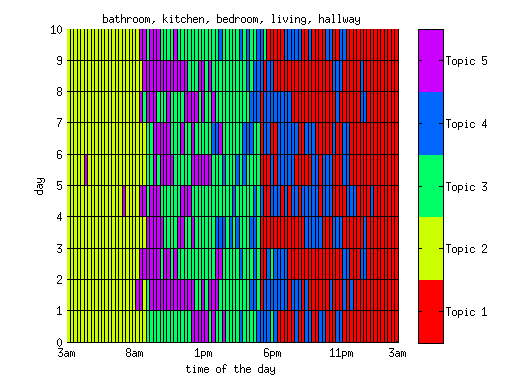
\includegraphics[width=\textwidth]{Pictures/TopDayHN2TS96k5Pois.png}
  \caption{Topic distribution for 10 days}
  \label{fig:PoisDay96}
 \end{subfigure}
 \begin{subfigure}[b]{0.45\linewidth}
  \centering
  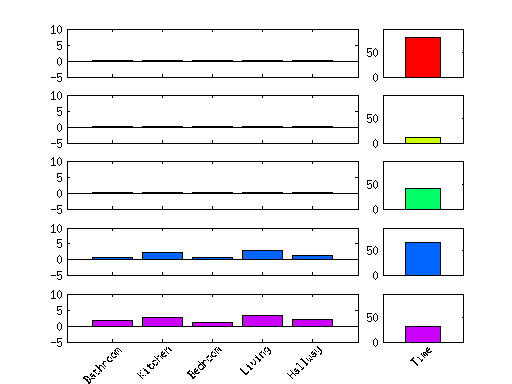
\includegraphics[width=\textwidth]{Pictures/TopVisuHN2TS96k5Pois.png}
  \caption{Visualization of the topics}
  \label{fig:PoisTopVisu96}
 \end{subfigure}
 \caption{Topic distribution per day and the Topic visualization for LDA-Poisson}
 \label{fig:Pois96}
\end{figure}


\paragraph{LDA-Gaussian 96 Time-slices and 5 Topics}
Figure \ref{fig:Gaus96} shows the outcome of the LDA-Gaussian model, $N=96$ and $k=5$. In the right figure (\ref{fig:GausTopVisu96}) on the x-axis again the 6 dimensions of the observations are shown. On the y-axis the mean value $\mu$ of the Gaussian distribution is shown and in the barchart the standard deviation $\sigma$ is given with a vertical black line. You can see that the red topic here has a high $\sigma$-value and captures all time-slice where no sensor data is measured. The purple topic seems to represent the 'Going to the toilet at night' topic. Here the mean value of the time is low and only a few sensor measurements are captured. You can see that this model captures more sophisticated topics, that represent more meaningful results.

\begin{figure}[h!]
 \centering
 \begin{subfigure}[b]{0.45\linewidth}
  \centering
  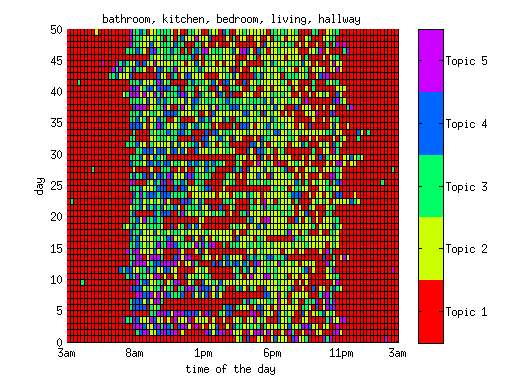
\includegraphics[width=\textwidth]{Pictures/TopDayTS96k5Gaus.png}
  \caption{Topic distribution for 10 days}
 \end{subfigure}
 \begin{subfigure}[b]{0.45\linewidth}
  \centering
  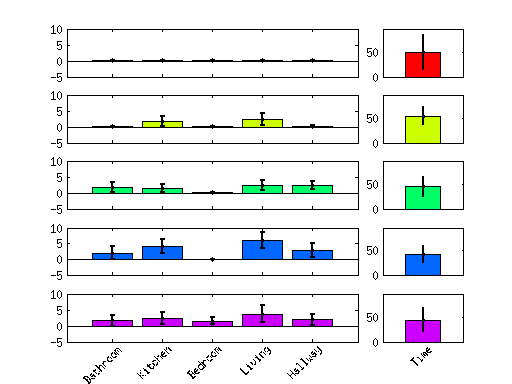
\includegraphics[width=\textwidth]{Pictures/TopVisuTS96k5Gaus.png}
  \caption{Visualization of the topics}
  \label{fig:GausTopVisu96}
 \end{subfigure}
 \caption{Topic distribution per day and the Topic visualization for LDA-Gaussian}
 \label{fig:Gaus96}
\end{figure}

\paragraph{LDA-Poisson 48 Time-Slices and 20 Topics}
In figure \ref{fig:Pois48} the outcome of the LDA-Poisson model is shown, where the amount of time-slices that is used is $N=48$ and the amount of topics is $k=20$. Again we have 6 dimension in the observations, but now we take a finer grid for the time dimension, which contains now $48$ time intervals, for every time-slice on a day one. We visualize the 10 most important topic, which are the topics with the highest $\alpha$-values. Time-slices that belong to a different topic than these 10 are marked with the color gray in the left images (\ref{fig:PoisTopVisu48}).
For the Bag-of-Word and the k-means model no reasonable results are found for these amount of time-slices and topics.	
\begin{figure}[h!]
 \centering
 \begin{subfigure}[b]{0.45\linewidth}
  \centering
  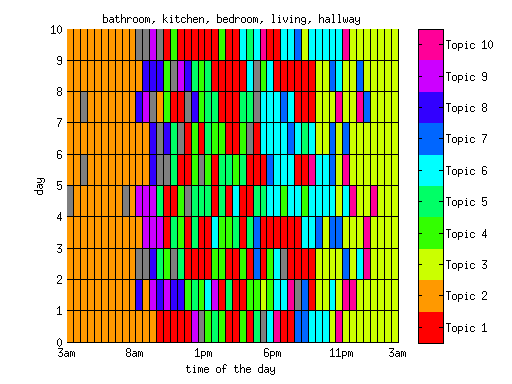
\includegraphics[width=\textwidth]{Pictures/PoisDayHN2TS48k20.png}
  \caption{Topic distribution for 10 days}
 \end{subfigure}
 \begin{subfigure}[b]{0.45\linewidth}
  \centering
  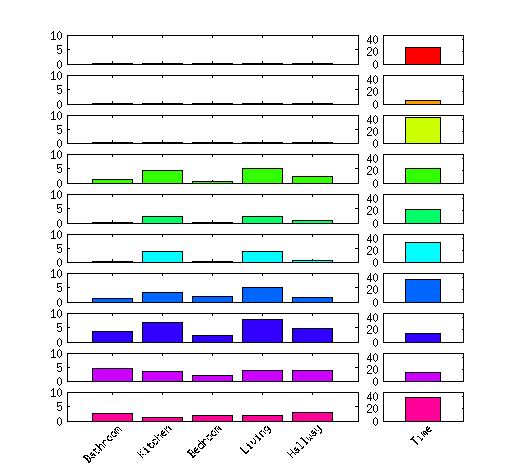
\includegraphics[width=\textwidth]{Pictures/PoisTopHN2TS48k20.png}
  \caption{Visualization of the topics}
  \label{fig:PoisTopVisu48}
 \end{subfigure}
 \caption{Topic distribution per day and the Topic visualization for LDA-Gaussian}
 \label{fig:Pois48}
\end{figure}

\paragraph{LDA-Gaussian 48 Time-Slices and 20 topics}
Figure \ref{fig:Gaus48} show the outcomes of the LDA-Gaussian model with $N=48$, $k=20$. Again only the 10 topics with the highest $\alpha$-value are shown.

\begin{figure}[h!]
 \centering
 \begin{subfigure}[b]{0.45\linewidth}
  \centering
  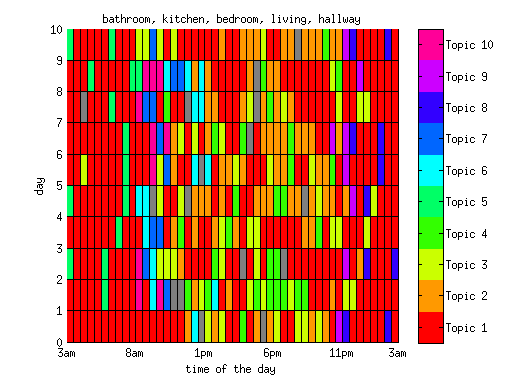
\includegraphics[width=\textwidth]{Pictures/GausDayHN2TS48k20.png}
  \caption{Topic distribution for 10 days}
 \end{subfigure}
 \begin{subfigure}[b]{0.45\linewidth}
  \centering
  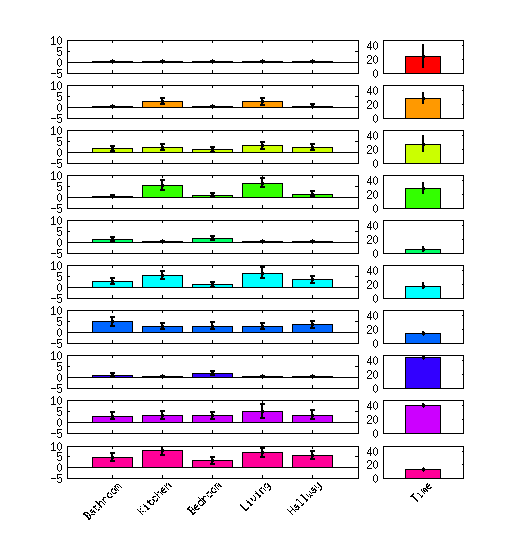
\includegraphics[width=\textwidth]{Pictures/GausTopHN2TS48k20.png}
  \caption{Visualization of the topics}
  \label{fig:GausTopVisu48}
 \end{subfigure}
 \caption{Topic distribution per day and the Topic visualization for LDA-Gaussian}
 \label{fig:Gaus48}
\end{figure}


\pagebreak


\subsection{Quantitative Results}
To see if our results not only hold on our training data we we wish to also find a high log-likelihood for a hold-out set. In this way we make sure that the model does not over-fit the data. So for a given hold-out set we can calculate the perplexity with 

\begin{equation}
 perplexity(D_{HOS}) = exp \left\{ - \frac{\sum_{m=1}^M \log p(\textbf{o}_d ) }{M*N} \right\}
\end{equation}

In the next experiments we use 10\% percent of our data as a hold-out set. We train the model on the rest of the data for different initialization values and calculate the perplexity for every run.

\paragraph{Different Sets of Data}
In figure \ref{fig:PerplGaus} the perplexity is shown for the 5 different data-sets gained from the 5 houses. Every run is performed ten times and we took the mean over these runs for every initialization of amount of topics $k$. Every run is initialized with 5 days.
The data sets vary in length, but as you can see in the figure, the amount of data is not necessary of influence how well the LDA-Gaussian model can be trained. Some data sets are much more stable than others and this is probably due to the way how regular peoples behavior is.

\begin{figure}[h!]
 \centering
 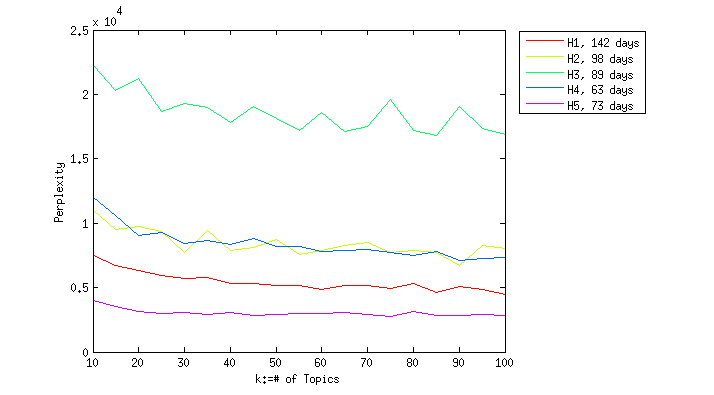
\includegraphics[width=0.7\textwidth]{Pictures/PerplGaus.png}
 \caption{Perplexity for different initializations of Topics for 5 different House}
 \label{fig:PerplGaus}
\end{figure}

\paragraph{Comparison LDA-Gaussian and LDA-Poisson}

To compare the two models with each other we drop the time dimensions in the observations and calculate the perplexity for the hold-out set with different amount of time-slices (figure \ref{fig:CompareTS}) and with different amount of topics (figure \ref{fig:CompareK}).
You can see that the LDA-Gaussian model outperforms the LDA-Poisson model for small amount of time-slices as well as for small amount of topics. When the amount of time-slices increases the performance of both models becomes similar to each other. 

\begin{figure}[h!]
 \centering
 \begin{subfigure}[b]{0.45\linewidth}
  \centering
  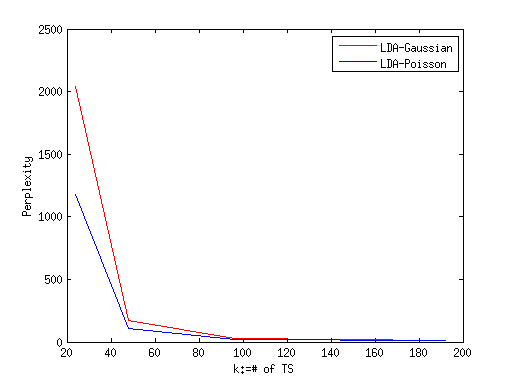
\includegraphics[width=\textwidth]{Pictures/CompareTSgausPois.png}
  \caption{Perplexity for LDA-Gaussian and LDA-Poisson with different amount of time-slices}
  \label{fig:CompareTS}
 \end{subfigure}
 \begin{subfigure}[b]{0.45\linewidth}
  \centering
  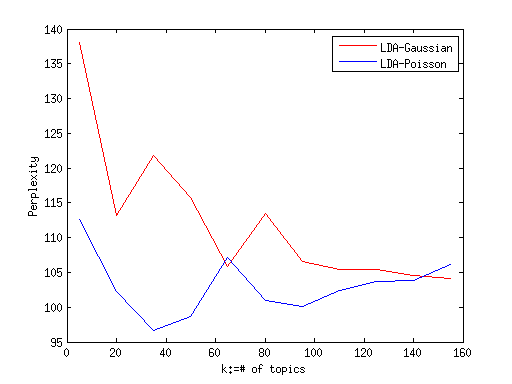
\includegraphics[width=\textwidth]{Pictures/CompareKgausPois.png}
\caption{Perplexity for LDA-Gaussian and LDA-Poisson with different amount of topics}
  \label{fig:CompareK}
 \end{subfigure}
 \caption{}
 \label{fig:Compare}
\end{figure}


\paragraph{Different length of time-slices}

In figure \ref{fig:PerplTS} we give the perplexity for different length of time-slices for the 5 Houses. We take a again the mean over 10 runs. We take for every house the same amount of days to train and test the data. We can see that with more time-slices the perplexity becomes lower for the hold-out set. For house $H2$ and $H4$ the perplexity is much better for a small amount of time-slices. The perplexities for these two houses drop much faster if the amount of time-slices increases.

\begin{figure}[h!]
 \centering
 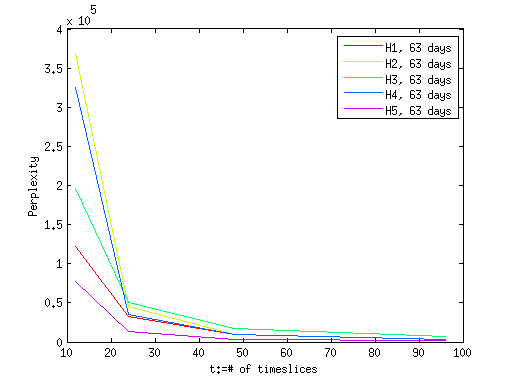
\includegraphics[width = 0.7\textwidth]{Pictures/PerplTS.png}
 \caption{Perplexity (x-axis) for the hold-out-set for different amount of time-slices (y-axis)}
 \label{fig:PerplTS}
\end{figure}


\pagebreak
 
%---------------------------------------DISCUSSION&CONCLUSION----------------------------------

\section{Discussion}
\label{sec:Disc}

\subsection{LDA with Bag-of-Words model}
Met de feature representation kunenn we uit BOW niks halen. Als de TS kleiner worden is er niet meer genoeg informatie beschikbaar om zinige informatie eruit te halen.
Smoothing moet worden gedaan.

With our feature representation we were not possible to find a good topic representation of the data. We see that the model works better if the amount of time slices gets bigger. Shorter time-slices means that the variance of the observation becomes not that high. Because it is not very likely that in a time-slice of one minute 20 or more sensor activations are received. At least not in our sensor data.  So if the size of time-slices is small, which equals a lot of time-slices per dat, the the amount of unique observations is reduced with respect to the amount of observations in the whole data set.\\
So it might be possible that the model will find a good topic representation with a bigger amount of time-slices or another feature representation.

\subsection{LDA with pre-clustering}
To use a cluster algorithm apriori does reduce the size of the 'Dictionary'. The LDA model then finds a better topic description of the data, but still there are some problems which makes it hard to get good results. First of all it is not so simple to find the best amount of clusters that should be used. And also the found clusters are not that good to use. Every 

\subsection{LDA-Poisson}
The Poisson distribution is not the best choice to model the time dimension. Nevertheless the outcome of the LDA-Poisson is still good and comparable with the LDA-Gaussian model.

\subsection{LDA-Gaussian}
We can see that the LDA-Gaussian model outperfoms the LDA-Poisson model if the amount of time-slices is small. This is due to the fact that if the time-slices are brought the amount of events counted in this time-interval can be high. The Poisson distribution will automatically have a brought variance for high values, which is not necessarily the case in the Gaussian distribution. The Gaussian distribution is more flexible. Which can also be seen in the fact that we are able to make use of the covariance between dimensions. We have not implemented it because to train this kind of model a lot of data need to be available.
Using the Gaussian distribution has another advantage. If for example another feature representation is used, which is not based on discrete values, the LDA-Gaussian model is still applicable.
\\

\section{Conclusion}
\label{sec:Conc}
In this thesis two novel models are represented which are based on the Latent Dirichlet Allocation model. Both models are applied to a real world sensor data, which is gained in the house of elderly people. With the models we are able to find behavior pattern in the data.
It is totally possible to find topics, given them a name is another difficulty

% We are not able to detect small activities, because in our data we group all sensors together that are located in the same room. We want to see if there is a behavior pattern on a more global way, that can be found regularly. Is there a topic distribution that returns frequently, can you see if it is a weekday or weekend? Wednesdays?

\appendix

\bibliography{research}{}
\bibliographystyle{plain}
% Misschien de newton Rhapson methode
% Overzicht van alle variabelen die zijn gebruikt

\end{document}